%% LyX 2.2.4 created this file.  For more info, see http://www.lyx.org/.
%% Do not edit unless you really know what you are doing.
\documentclass[english]{book}
\usepackage[T1]{fontenc}
\usepackage[latin9]{inputenc}
\usepackage[paperwidth=10.5cm,paperheight=10.5cm]{geometry}
\setlength{\parskip}{\smallskipamount}
\setlength{\parindent}{0pt}
\synctex=-1
\usepackage{array}
\usepackage{booktabs}
\usepackage{multirow}
\usepackage{graphicx}
\PassOptionsToPackage{normalem}{ulem}
\usepackage{ulem}

\pagenumbering{gobble}

\makeatletter

%%%%%%%%%%%%%%%%%%%%%%%%%%%%%% LyX specific LaTeX commands.
%% Because html converters don't know tabularnewline
\providecommand{\tabularnewline}{\\}

%%%%%%%%%%%%%%%%%%%%%%%%%%%%%% Textclass specific LaTeX commands.
\newenvironment{lyxlist}[1]
{\begin{list}{}
{\settowidth{\labelwidth}{#1}
 \setlength{\leftmargin}{\labelwidth}
 \addtolength{\leftmargin}{\labelsep}
 \renewcommand{\makelabel}[1]{##1\hfil}}}
{\end{list}}

\@ifundefined{date}{}{\date{}}
\makeatother

\usepackage{babel}

\begin{document}

\begin{picture}(0,0)
   \put(-36,-253){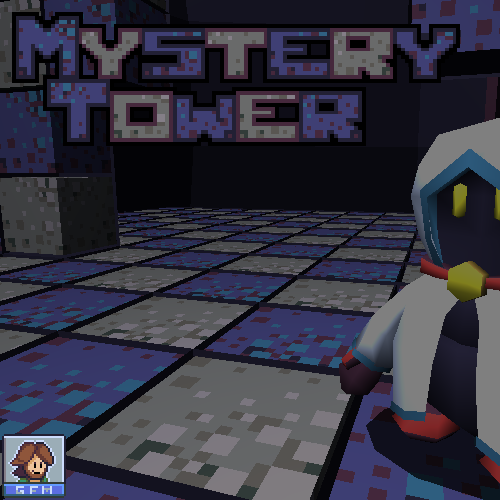
\includegraphics[width=10.5cm,keepaspectratio]{imgs/cover.png}}
\end{picture}

\cleardoublepage{}

\section*{The... story?}

You find yourself trapped in a tower.

Who trapped you there?

Why?

Where is this tower?

Did the dev just made all this up to pretend the game has some sort
of story?

It's a mystery...

\cleardoublepage{}

\section*{Legal disclaimer}

This game is based on Catherine, developed by Atlus. This game is
not affiliated with, endorsed by, sponsored by or specifically approved
by Atlus, SEGA, or their partners.

This is a homage made by a fan who has spent too much time playing
that game. If you enjoyed this game, please consider supporting Atlus
and SEGA by purchasing Catherine Classic, for PC, or Catherine: Full
Body, for consoles.\pagebreak{}

\section*{About the game}

Mystery Tower is a puzzle game in which the player is tasked with
climbing towers.

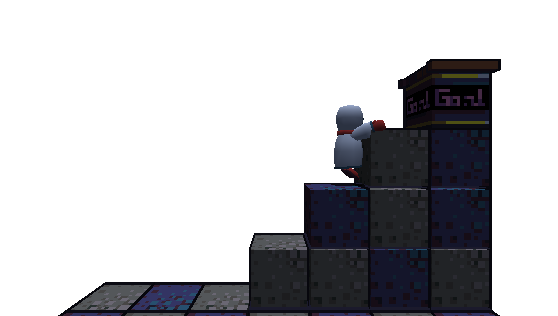
\includegraphics[width=0.75\paperwidth]{imgs/000-climb-to-goal}

\pagebreak{}

You control a nameless character able to climb, push and pull blocks.
Use these actions to build stairways and bridges, and even to demolish
part of the tower, creating paths toward the goal at the top.

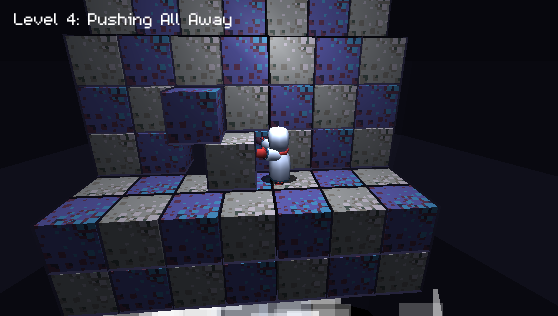
\includegraphics[width=0.75\paperwidth]{imgs/000-game-example}

\pagebreak{}

\subsection*{Controls}

These are the default game controls, which can be remaped from the
Options menu.

\begin{tabular*}{0.75\paperwidth}{@{\extracolsep{\fill}}>{\centering}m{0.175\textwidth}>{\centering}m{0.175\textwidth}>{\centering}m{0.175\textwidth}>{\centering}m{0.175\textwidth}}
\toprule 
Action & Keyboard & Gamepad & Alt.\tabularnewline
\midrule
\midrule 
\multirow{1}{0.175\textwidth}{Movement} & WASD & Left analog & Gamepad

D-Pad\tabularnewline
\midrule 
Push/Pull & Spacebar & Button0 & \tabularnewline
\midrule 
Ledge drop & Left shift & Button1 & \tabularnewline
\midrule 
Camera & UHJK & Right analog & Right mouse\tabularnewline
\midrule 
Reset & R &  & \tabularnewline
\midrule 
Pause & Escape & Start & \tabularnewline
\bottomrule
\end{tabular*}

\pagebreak{}

\section*{Block types}
\begin{lyxlist}{00.00.0000}
\item [{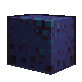
\includegraphics[viewport=0bp 30bp 82bp 82bp,width=0.2\linewidth]{imgs/002-default-block}}] A
regular block with no special traits
\item [{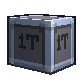
\includegraphics[viewport=0bp 41bp 82bp 82bp,width=0.2\linewidth]{imgs/003-heavy-block}}] A
heavy block that takes longer to push
\item [{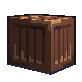
\includegraphics[viewport=0bp 41bp 82bp 82bp,width=0.2\linewidth]{imgs/004-breakable-block}}] A
fragile block that breaks if you walk over it twice
\item [{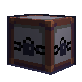
\includegraphics[viewport=0bp 41bp 82bp 82bp,width=0.2\linewidth]{imgs/005-imovable-block}}] An
imovable block. It won't budge, but you could cause it to fall...
\item [{
\includegraphics[viewport=0bp 41bp 82bp 82bp,width=0.2\linewidth]{imgs/006-goal-block}}] The
goal block. Reach this to end a level\pagebreak{}
\end{lyxlist}

\subsection*{Climbing tips}

\begin{tabular*}{0.8\textwidth}{@{\extracolsep{\fill}}>{\centering}m{0.4\textwidth}>{\centering}m{0.4\textwidth}}
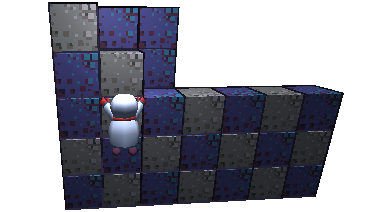
\includegraphics[width=0.38\textwidth]{imgs/007-ledge} & You can drop to, and move around ledges\tabularnewline
\end{tabular*}

\bigskip{}

\begin{tabular*}{0.8\textwidth}{@{\extracolsep{\fill}}>{\centering}m{0.4\textwidth}>{\centering}m{0.4\textwidth}}
You can push multiple blocks at once. The speed will be limited by
the heaviest block, though & 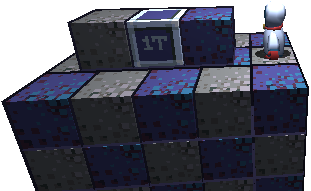
\includegraphics[width=0.38\textwidth]{imgs/010-push-many}\tabularnewline
\end{tabular*}

\pagebreak{}

~

\vspace{0.12\paperheight}

\begin{tabular*}{0.8\textwidth}{@{\extracolsep{\fill}}>{\centering}m{0.4\textwidth}>{\centering}m{0.4\textwidth}}
Blocks will start falling if there's no block supporting it & 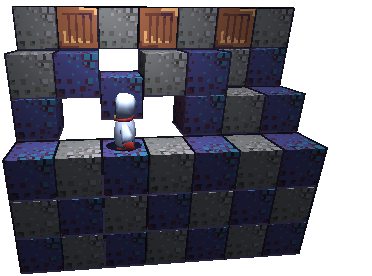
\includegraphics[width=0.38\textwidth]{imgs/008-dropping-blocks}\tabularnewline
\end{tabular*}

\vspace{0.1\paperheight}

\begin{tabular*}{0.8\textwidth}{@{\extracolsep{\fill}}>{\centering}m{0.4\textwidth}>{\centering}m{0.4\textwidth}}
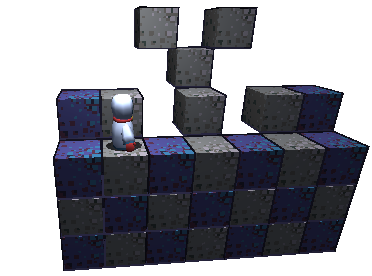
\includegraphics[width=0.38\textwidth]{imgs/009-block-edge} & A block only needs to be touching another's edge to be supported by
it\tabularnewline
\end{tabular*}

\pagebreak{}

\section*{Troubleshooting}
\begin{itemize}
\item If the input binding becomes terribly broken, reset the configuration:
\begin{itemize}
\item Use the option ``Reset Config and Play'' on the itch app
\item Launch the game from a command-line with the option ``\textendash reset-config''
\item On Windows, you may also use the script reset-config.bat to launch
the game and reset the configurations
\end{itemize}
\end{itemize}
\pagebreak{}

\null

\pagebreak{}

\section*{Credits, Acknowledgments and stuff}
\begin{itemize}
\item Made with Unity, Blender, LMMS, BFXR, GIMP, VIM, Python and Audacity
\item 32 color palette by DawnBringer:
\begin{itemize}
\item {\tiny{}\uline{http://pixeljoint.com/forum/forum\_posts.asp?TID=16247}}{\tiny\par}
\end{itemize}
\item ``Everything else'' (code, graphics, models, animations, song) by
GFM
\item Project hosted on Github. It's Open Source, so feel free to check
it out at:
\begin{itemize}
\item {\tiny{}\uline{https://github.com/SirGFM/FallingBlocks}}{\tiny\par}
\end{itemize}
\item Game freely available on itch.io, at:
\begin{itemize}
\item {\tiny{}\uline{https://gfm.itch.io/mystery-tower}}{\tiny\par}
\end{itemize}
\end{itemize}
\pagebreak{}

Back in January of 2016, I started making my next ``non-game jam''
game, after JJAT. After almost four years of working on and off on
that project, in July of 2019 I ended up pausing that project to start
Mystery Tower.

What I initially envisioned as being a three months long project ended
up taking almost a full year. I learned a lot of things, had to rewrite
the project once, used an effin' third-party engine, complained a
lot... But had tons of fun!

If you've read this far, thank you! I must also thank friends and
family for always supporting my doing these silly projects, even though
I'm not even that vocal about it (I think?).

Also, special thanks to Pirata/pool\_shark, who pretty much tested
every version of the game, and helped a lot in defining its current
form.

\pagebreak{}

Also extra special thanks to everyone in SRL Mystery Game Tournament
(MT), the Mystery Fun House crew, and the blind race/mystery community
in general!

Having submitted a game for a previous MT and really enjoying taking
part on these events, I made this game specifically so it were viable
for blind racing, and so I could submit it to another MT.

All the feedback I got after submitting, specially from BlasphemousRoar
and Exuno, were invaluable! And then, seeing it being raced in MT15's
finals was a blast!

So thanks everyone!

\pagebreak{}

\null

\pagebreak{}

\begin{picture}(0,0)
   \put(-54,-253){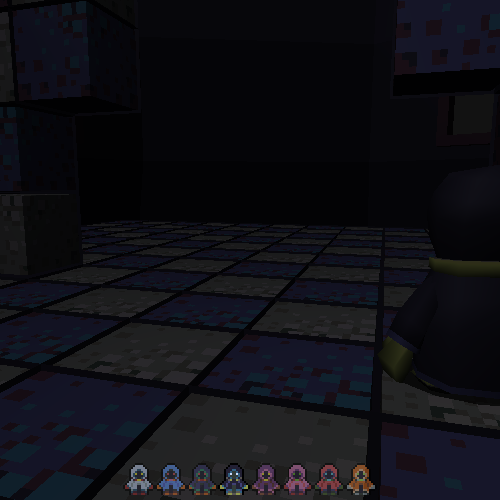
\includegraphics[width=10.5cm,keepaspectratio]{imgs/back-cover.png}}
\end{picture}

\end{document}
